\documentclass[11pt]{article}   	% use "amsart" instead of "article" for AMSLaTeX format
\usepackage[margin=1in]{geometry}                		% See geometry.pdf to learn the layout options. There are lots.
\geometry{letterpaper}                   		% ... or a4paper or a5paper or ... 
%\geometry{landscape}                		% Activate for rotated page geometry
\usepackage[parfill]{parskip}    		% Activate to begin paragraphs with an empty line rather than an indent
\usepackage{graphicx}				% Use pdf, png, jpg, or eps§ with pdflatex; use eps in DVI mode
								% TeX will automatically convert eps --> pdf in pdflatex		
\usepackage{amssymb}


%\usepackage{setspace}
%\doublespacing


\title{ChE 696 Final project: Modeling explosive percolation under local rules}
\author{Shannon Moran \\ Fall 2018}
\date{}

\begin{document}
\maketitle

%%% INTRODUCTION
\section{Introduction}

For this class project, I wanted to try to replicate a peer-reviewed publication. My thesis research didn't lend itself easily to a topic relevant to the class. I had explored explosive percolation for a prior class project, and decided to pick a recent paper from the field to replicate.

``Explosive'' percolation is so named because of the sudden growth in the largest cluster in the system. While percolation on a random graph will have incrementally-growing cluster sizes, explosive percolation is the result of edge-addition rules that bias the system towards formation of smaller clusters. Eventually, the ``smallest'' cluster that can be formed by an edge addition is the combination of two large clusters, leading to ``explosive'' growth. These edge-addition rules can be called ``competitive'', and the field has explored a number of different competitive edge-addition algorithms and their impact on the growth and critical behavior of network systems.

In this report, I chose to replicate the work done by Trevelyan \textit{et al.} \cite{DPR_paper}. This paper introduces a new percolation algorithm called the ``Degree product rule'' (DPR) in which network edges are added based entirely on local rules.

This DPR  algorithm is contrasted with the Erd\"{o}s-R\'{e}nyi (ER) and Achlioptas growth process (AP). Networks generated by ER rules are purely random, with a Poisson distribution of edges off each node (i.e. no local or global preference). In contrast, the AP edge-addition rules are based on global rules and lead to explosive percolation \cite{AP_paper}. The authors assert that their DPR method leads to explosive percolation in a way that is entirely derived from local rules. Additionally, they assert that these systems exhibit a second-order phase transition for small $m$ and a first-order transition for global $m$.

In this project, I've been able to replicate the explosive percolation algorithms discussed. However, I had difficulty precisely replicating the critical behavior due to computational and time limitations inherent to a class versus research project. However, I am confident that with additional time/compute resources I would be able to get the sufficient statistics required for deriving the critical exponents.

%%% METHODS
\begin{figure}[t]
\begin{center}
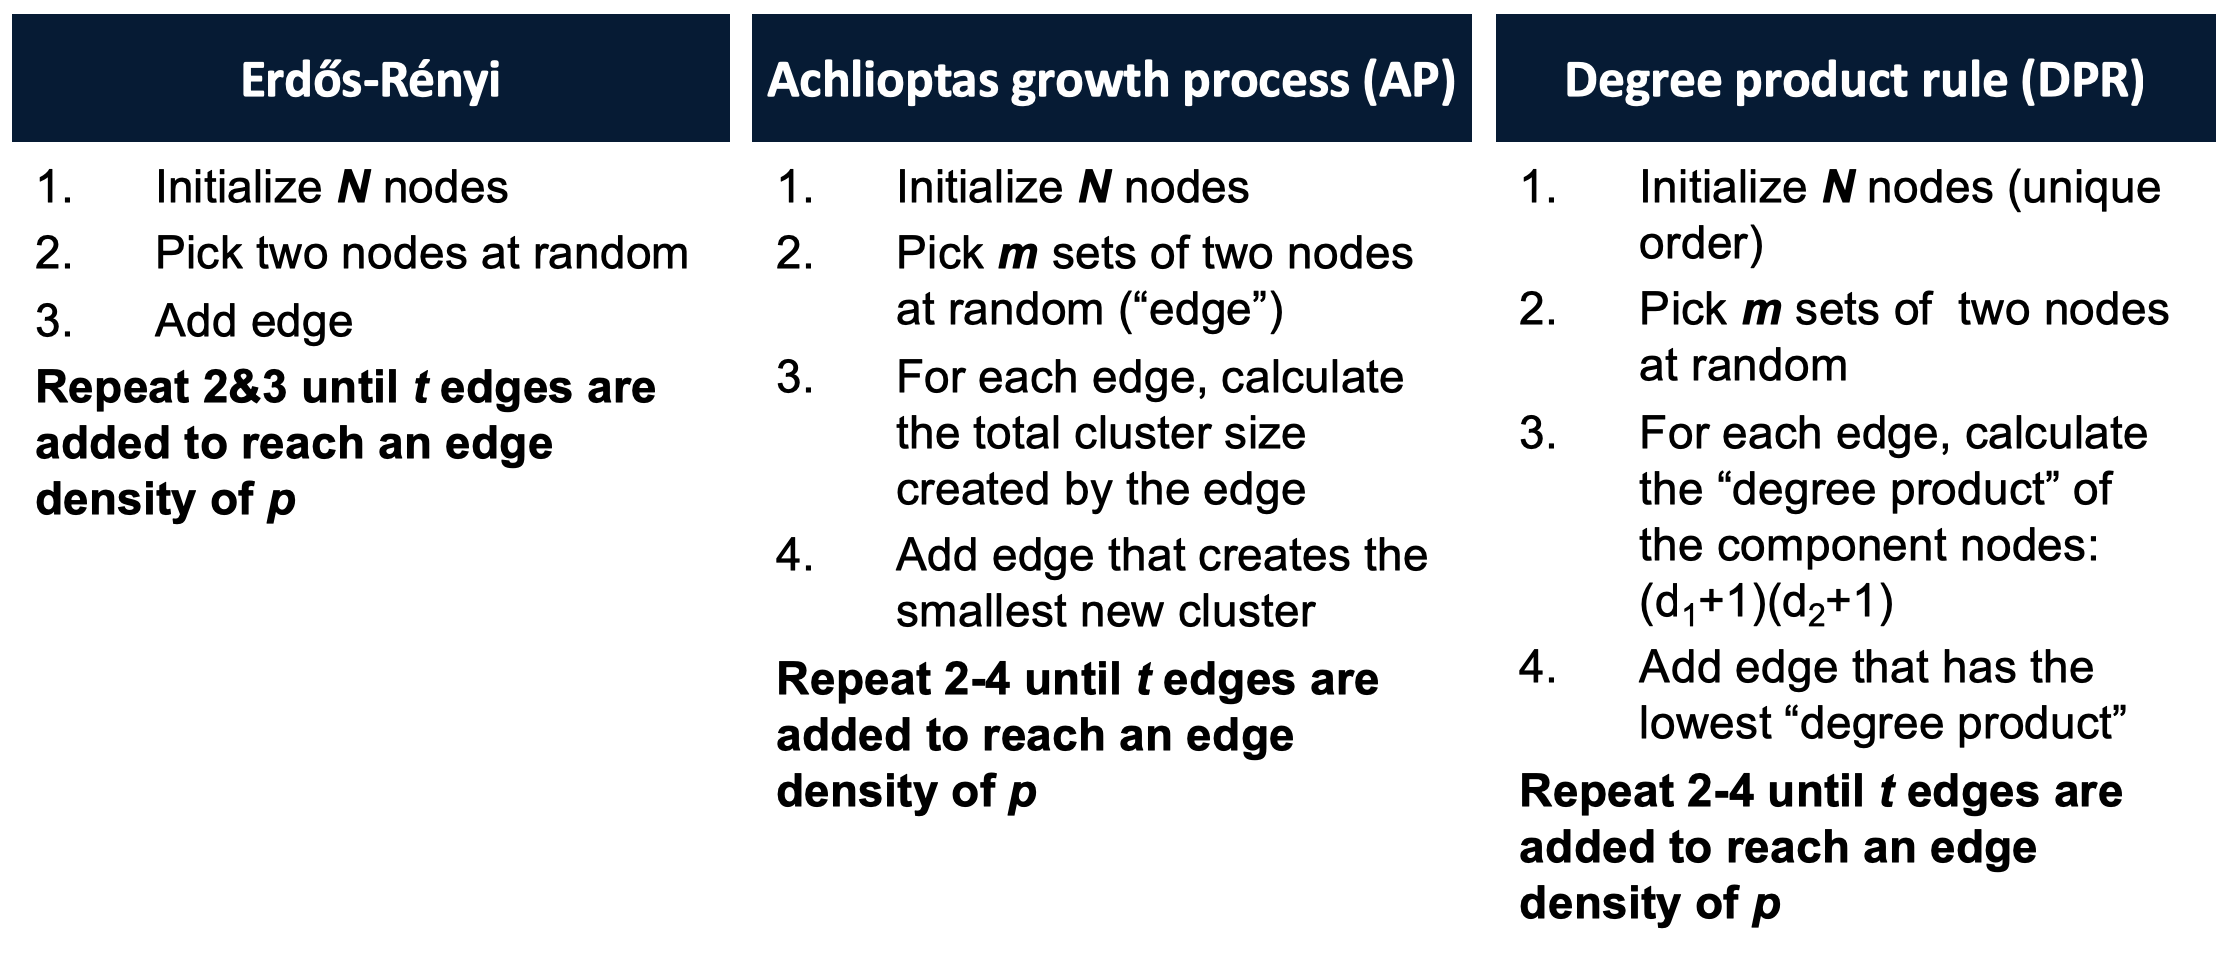
\includegraphics[width=1.0\textwidth]{fig/algorithms.png}
\caption{Summary of percolation algorithms replicated in this study. DPR was the novel contribution by Trevelyan \textit{et al.} \cite{DPR_paper}.}
\label{fig:algorithms}
\end{center}
\end{figure}

\begin{figure}[t]
\begin{center}
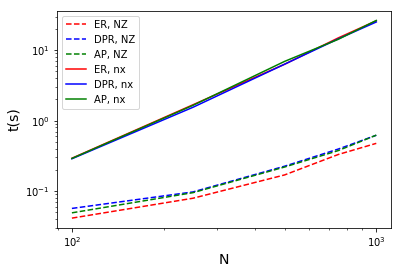
\includegraphics[width=0.65\textwidth]{fig/time.png}
\caption{Time to generate graphs of size N and edge density $p=1$ using the Newman-Ziff (NZ) algorithm or Networkx (nx) built-in methods. Using the NZ implementation delivered over an order of magnitude speed-up.}
\label{fig:time}
\end{center}
\end{figure}

\section{Methods}
\subsection{Percolation algorithms}
A summary of the percolation algorithms implemented in this project are summarized in Figure \ref{fig:algorithms}. I used Python to implement these algorithms.

Initially, I set up these algorithms up without any packages outside the core scientific computing stack. However, I then refactored my code to use the \verb|networkx| graph generation methods. This didn't significantly change the performance, but allowed me to use the package's built in clustering algorithms. Ultimately, this might have been a bad thing. I compare these built-in methods to more efficient algorithms below.

\subsection{Finding clusters sizes on the network}

I initially used built-in methods in the \verb|networkx| package to ``quickly'' calculate the cluster sizes in the graph at each step (\verb|node_connected_component| and \verb|connected_component_subgraphs|). While I knew calculating the cluster sizes at each step was computationally expensive, I assumed that using these generator methods wouldn't slow down my work too badly. I was wrong.

\textbf{Implementing the Newman-Ziff (NZ) algorithm significantly sped up my work \cite{NZ_paper}.} The magnitude of this jump should not have been as surprising as it was. While $N=1e3$ was previously the largest network size I could comfortably run on my laptop, NZ enabled me to run $N=1e4$ in times that were reasonable for a class project. The difference is shown in Figure \ref{fig:time}.

The canonical NZ algorithm has: (1) pointer array for tracking cluster size and membership, (2) random order of site percolation, (3) list of nearest neighbors for each site. I had to modify the algorithm on all three counts to suit this problem. 

(1) Array for tracking cluster size and membership: I chose to code this project up in Python, as it's the language I'm most fluent with. I'd also wanted the chance to work with the \verb|networkx| package more extensively. However, the concept of a ``pointer'' doesn't exist in python, nor can one have an empty array. I eventually settled on initializing a size $N$ array of \verb|NaN| to track cluster membership. This then led to some later-on creativity in calculating max cluster size without introducing another python package (\verb|pandas|).

(2) Order of site percolation: In the canonical NZ algorithm, the site percolation order is set from the beginning. While this could also be the case for ER percolation, DPR and AP percolation steps are dependent on the structure of the network at each timepoint. To do this cleanly, I broke the core parts of the NZ algorithm into a look-up step (\verb|NZ_root_value|) to compare cluster sizes, then an update step (\verb|NZ_update|) to reflect the updated network structure after the addition of the ``winning'' edge. 

(3) Nearest neighbors: In graph percolation, the neighbors will be dependent on the edges added during the network formation. Here, I actually had it easier than site percolation; since each prior step of the algorithm will track which cluster a node is in, a node I'm proposing adding will only be in one cluster. No need to compare neighbors!
 

\subsection{Finding the largest cluster size jump}
The authors used the largest jump in cluster size as a preliminary order parameter for their systems. While the authors didn't mention how they approached this, I implemented a simple binary search to scan the percolation simulation.  




%%% RESULTS
\section{Results}

\subsection{Replicating network structure in the different percolating systems}

\begin{figure}[t]
\begin{center}
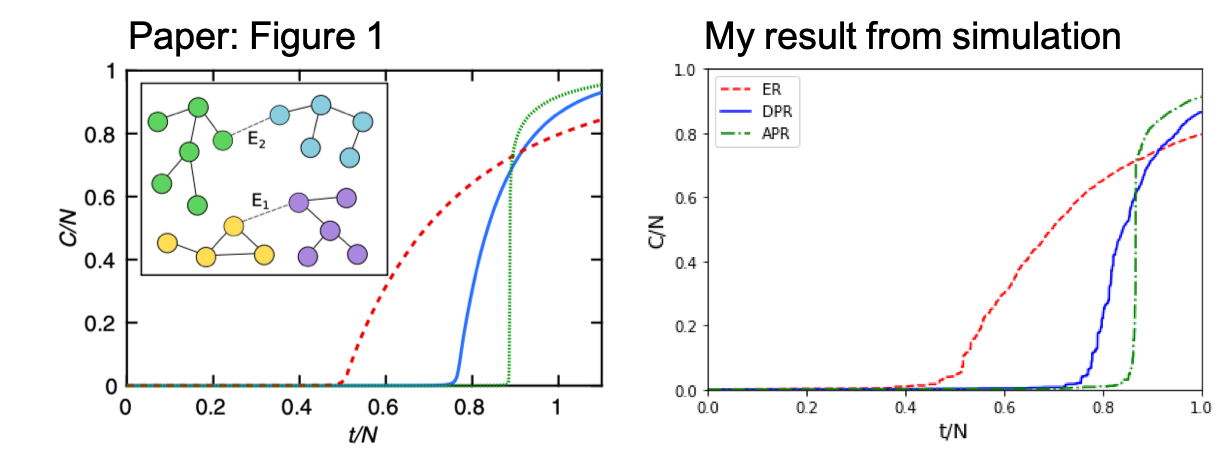
\includegraphics[width=\textwidth]{fig/fig1_comparison.png}
\caption{Relative size of the largest cluster ($C/N$) at scaled time $p=(t/N)$. Version from paper calculated from $N=3.6e5$ nodes. My result generated from $N=1e4$. Relative trends between algorithms and absolute location of percolation transitions are replicated by my simulations, despite the lower system size.}
\label{fig:fig1}
\end{center}
\end{figure}

The paper first characterizes the explosive (or not) percolation of the varying network algorithms by plotting the relative size of the largest cluster ($C/N$) as $t$ edges are incrementally added to the cluster until the edge density $p=1$. As shown in Figure \ref{fig:fig1}, my implementation is able to replicate this behavior.

My curves look slightly less smooth than those in the publication, as my system size has approximately 10x fewer nodes. However, this critical behavior will be independent of system size-- so I am able to replicate the onset of percolation and the general critical behavior. These curves also look significantly smoother than those ones generated at $N=1e3$, which were shown in my presentation.

\begin{figure}[t]
\begin{center}
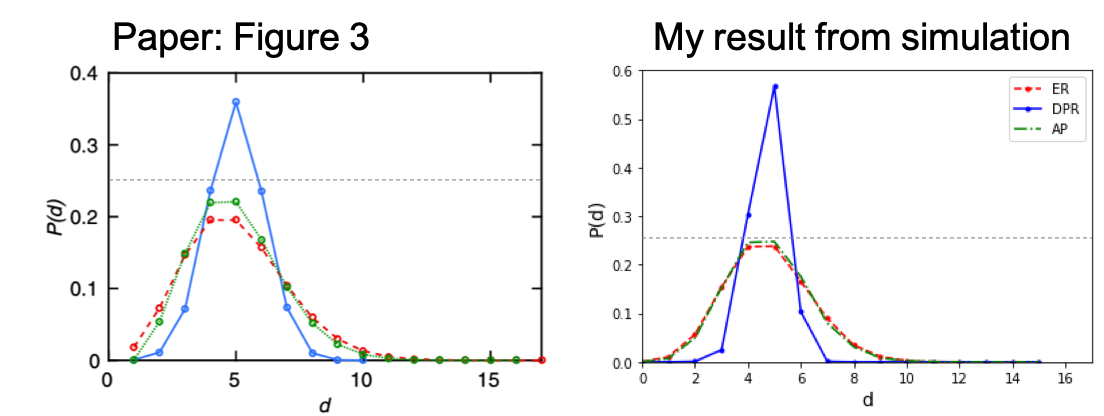
\includegraphics[width=\textwidth]{fig/fig3_comparison.png}
\caption{The degree distributions at $p=5$ for ER, DPR, and AP processes ($m=2$ for the later two). Publication graph calculated from $N=1.7e4$. My result generated from $N=1e4$. Grey dashed line added at $P(d)=0.25$ to serve as a guide for the eye between the two graphs, given the different $y$-scales.}
\label{fig:fig3}
\end{center}
\end{figure}

Next, I wanted to check that my algorithms were generating the correct degree distribution across nodes in the system, as shown in Figure \ref{fig:fig3}. Interestingly, I ended up with a much higher percentage of nodes with the degree distribution at the system average ($p=5$) than paper found. While my system size was on par with that simulated in the paper, given the stochastic nature of these systems I suspect the publication's graph was averaged over multiple replicates. Due to time constraints, I only ran one replicate for all graphs shown.

This replicate issue will rear its head in the next section.


\subsection{Calculating critical exponents in the system requires more statistics}

The need for replicates is immediately apparent in Figure \ref{fig:fig2}. Here, the authors sought to characterize the critical behavior by looking at the largest jump in the largest cluster size ($\Delta C_{max}/N$) for different system sizes and algorithm design choices.

Because these algorithms do have some randomness in the edge addition process, each data point shown in Figure \ref{fig:fig2} is only one sample in a statistical space. By running replicates (5 more? 10?) and taking the average, I would expect to see something more in line with the figure found by the authors. Given this, I'm also very surprised that the authors don't show any error bars on their plot. I'm encouraged that I would be able to replicate these critical exponents with more samples, as my results are in the same order of magnitude as those found by the authors.

While I was able to generate plots out to $N=1e5$, doing so in addition to $N=1e4$ and below/in-between was prohibitively time-expensive. Thus, my plots only go out to $N=1e4$. This is why people do these sorts of things as research problems, and not just class projects.

(Note that I did not implement global searches to replicate the AP and $m=$global aspects of Figure \ref{fig:fig2}. That would be an interesting challenge to implement efficiently.)

\begin{figure}[t]
\begin{center}
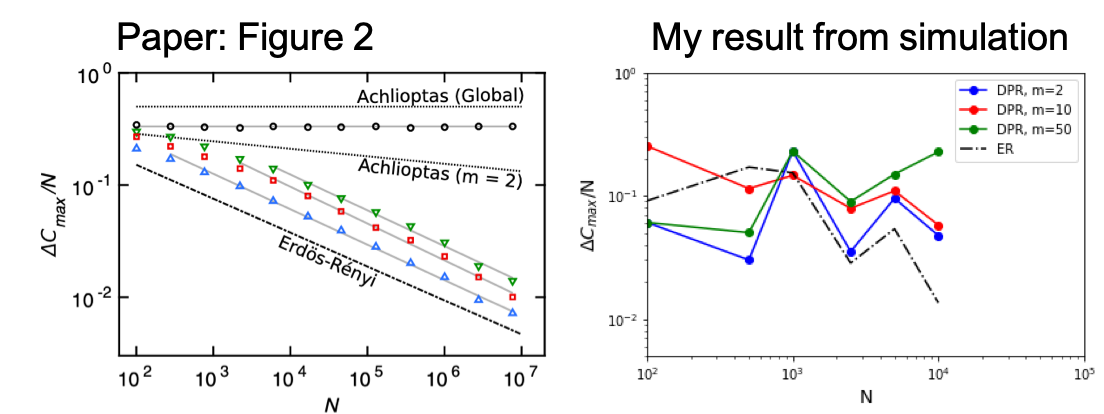
\includegraphics[width=\textwidth]{fig/fig2_comparison.png}
\caption{The average maximum jump in the order parameter as a function of system size for the DPR process with 2, 10, and 50 choices ($m$). Assumed $p=1.0$; value not provided in published text. Note the difference in x-axes.}
\label{fig:fig2}
\end{center}
\end{figure}

For calculating the critical exponents, both my system size and lack of replicates again presented issues. However, I was able to replicate the magnitude and trends of mean cluster size $S$ and largest cluster $C/N$ versus system size N (Figure \ref{fig:fig4}).

\begin{figure}[t]
\begin{center}
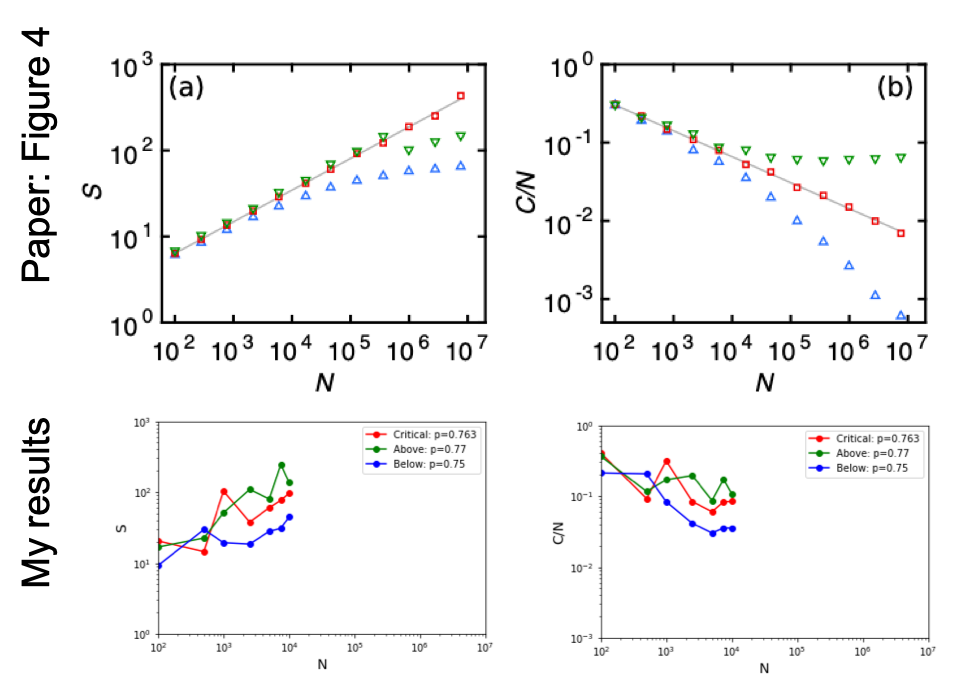
\includegraphics[width=\textwidth]{fig/fig4_compiled.png}
\caption{Finite-size scaling for the critical exponents $\beta/\nu$ and $\gamma/\nu$ of the DPR process. Mean cluster size $S$ and largest cluster $C/N$ is plotted versus system size $N$. Assumed value of $m=2$, not provided in published work. Note that x-axes are kept the same, even though my results do not extend to the same system sizes studied in the publication.}
\label{fig:fig4}
\end{center}
\end{figure}


%%% CONCLUSIONS
\section{Conclusions and next steps}
Overall, I was able to replicate (or get directionally close to) the main results found in this paper.
However, my replication of the critical behavior was limited by the size of the systems I was able to run within a reasonable amount of time and without further re-writing of this code into a lower-level language (e.g. \verb|C|/\verb|C++|).

In addition to code efficiency, my results would benefit from replicates. Due to time constraints, I only ran one replicate at each network size for each graph.

\textbf{Next steps}: The \verb|networkx| Python package is the ``gold standard'' for network analysis in Python.
However, it does not yet have an implementation of the Newman-Ziff algorithm for tracking cluster size organically.
I was able to find another open-source python package, \verb|pypercolate|, that has an implementation of the NZ algorithm.
However, it looks like the package hasn't been maintained in the last 3 years. Additionally, it appears to be designed for very vanilla percolation. I envision an implementation closer to mine that would allow for easy testing of competitive percolation methods where each step depends on the network structure. 

My implementation of the percolation algorithms is already integrated into how \verb|networkx| handles graphs. Over winter break, I intend to clean this up and submit a pull request to begin the process of adding this to \verb|networkx|. (And it will be my first non-Glotzer group open source contribution!)
As the scientific community moves towards Python as our testing ground, having a robust Python implementation of NZ readily available would be valuable. 
In particular, having an implementation of NZ in such a widely-used package as \verb|networkx| would lower the barrier to percolation newcomers adopting it.

\section{Code and reproducability}
All code for this project is contained in two Jupyter notebooks accompanying this final report.

\newpage
\bibliographystyle{unsrt}
\bibliography{citations}

\end{document}  